\section{Server Configuration}
\label{section:server}
This should be a short (break) section, in which I showcase the dashboard for the project on the Adafruit server and discuss a bit about grouping on Adafruit. Figure \ref{fig:dashboard} illustrates the dashboard design for this project. Dashboard design is easy and straightforward, so no further explanation is required.
\begin{figure}
    \centering
    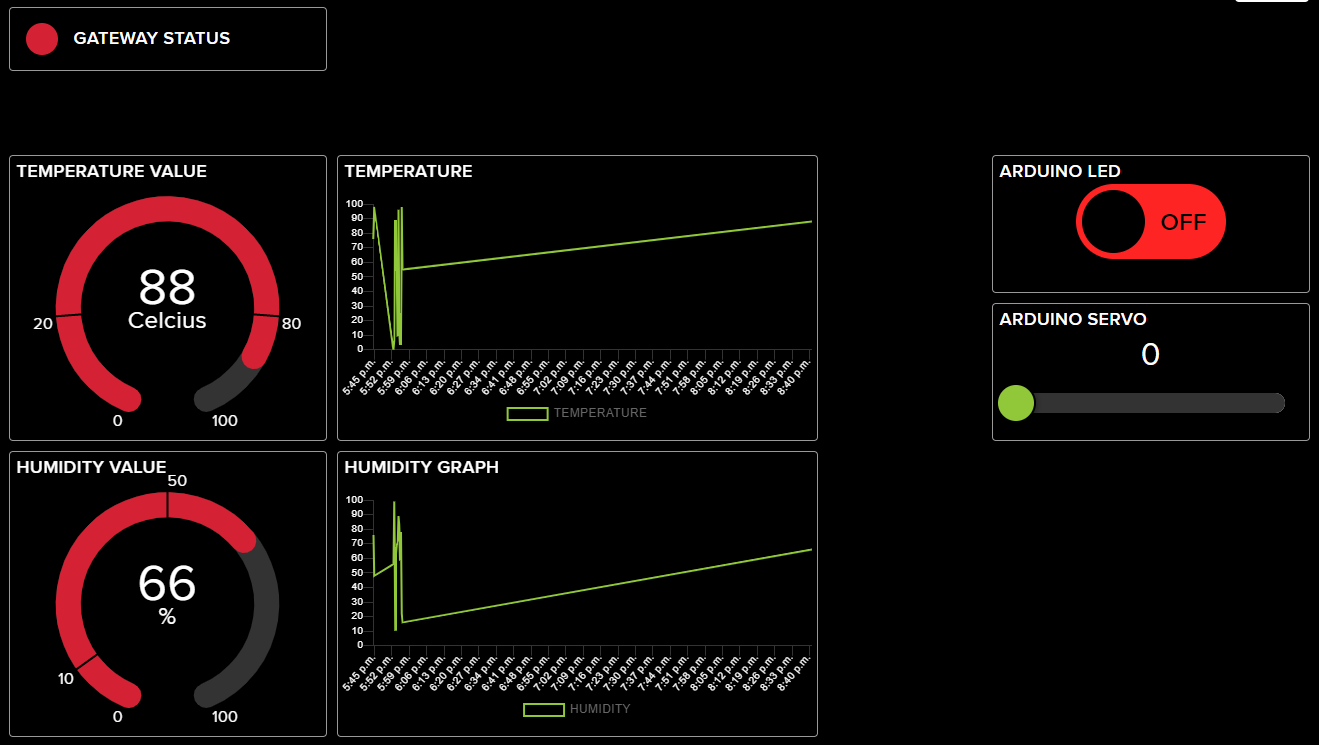
\includegraphics[scale=0.45]{screenshots/dashboard.png}
    \caption{Dashboard}
    \label{fig:dashboard}
\end{figure}

Figure \ref{fig:groups} captures the grouping feature of the Adafruit IO. Currently I have 2 groups, 1 is created default by the server, and 1 for this project. Grouping makes related topics more organized and eases the management of users. When a topic is assigned to a group other than the Default group, its proper name is prefix with its group name and a colon. 
\begin{figure}
    \centering
    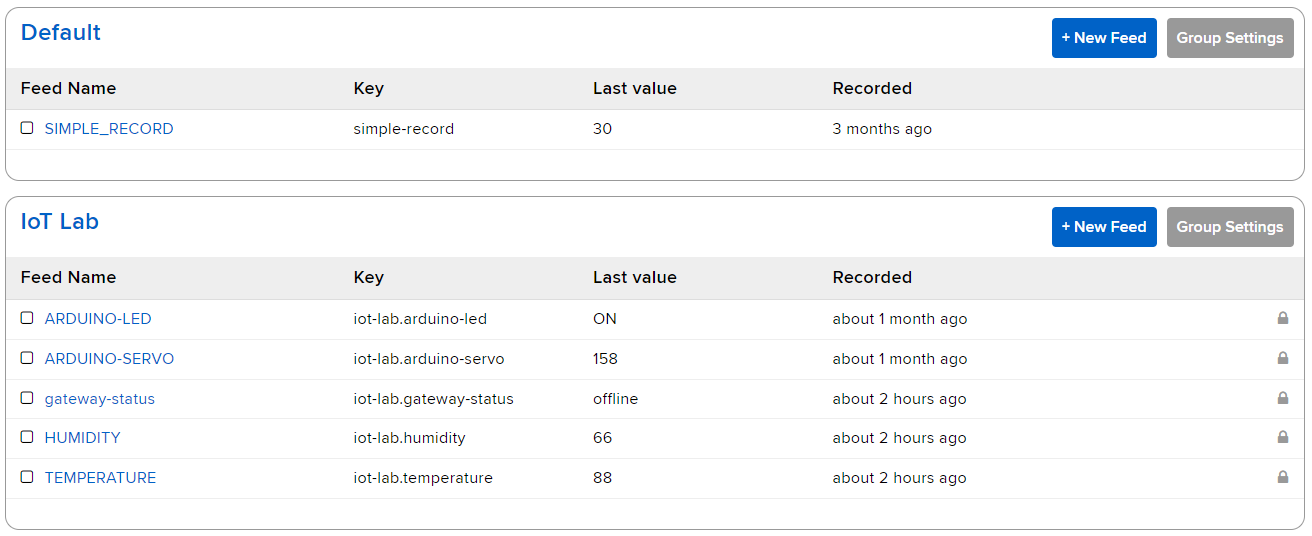
\includegraphics[scale=0.45]{screenshots/groups.png}
    \caption{Adafruit Grouping}
    \label{fig:groups}
\end{figure}
\clearpage